\documentclass[10pt,conference]{IEEEtran}
\usepackage{amsmath,amssymb}
\usepackage{graphicx}
\usepackage{booktabs}
\usepackage{hyperref}
\usepackage[font=footnotesize]{caption}
\graphicspath{{../results/}}

\begin{document}

\title{Critic-Free Group-Relative Policy Optimization\\for Anti-Sway Control of a Double-Pendulum Crane}

\author{\IEEEauthorblockN{Rupesh (B24CM1052)}
\IEEEauthorblockA{GitHub: \url{https://github.com/Zephyr-sue/rl_crane_antisway}}}

\maketitle

\begin{abstract}
We formulate anti-sway transport with an overhead crane, where a trolley carries a hook and a payload (a double pendulum), as a continuous-control RL problem. Payload mass, cable lengths, initial sway and wind gusts are randomized. We adapt \emph{Group Relative Policy Optimization} (GRPO)~\cite{grpo}, originally proposed for LLM reasoning, to physical control. GRPO has no value network: $G$ rollouts replay the \emph{same} randomized scenario on a GPU-batched simulator and serve as each other's baseline. We evaluate on 8 test conditions, including out-of-distribution plants and doubled gusts. GRPO succeeds in 93--97\% of random scenarios across 3 seeds. PPO with a learned critic reaches 77--94\%, and the RBF neural-network adaptive controller of~\cite{qiang2021} reaches 62\%. GRPO settles fastest and is most robust to gusts, while PPO needs $100\times$ fewer samples and generalizes better to unseen plants.
\end{abstract}

\section{Problem and Environment}
\textbf{Dynamics.} The state is $q=[x,\theta_1,\theta_2]$: trolley position, hook angle and payload angle. The Euler--Lagrange equations $M(q)\ddot q = F(q,\dot q) + \tau$ are taken from~\cite{qiang2021}, with viscous damping. They are integrated with RK4 at $\Delta t=0.02$\,s and are valid for large angles. A horizontal gust $F_d$ on the payload enters through $\tau = J^\top F_d = F_d[1,\,L_1\cos\theta_1,\,L_2\cos\theta_2]^\top$. Tests check energy conservation without damping (drift $<10^{-3}$) and that the energy change equals the gust's work.

\textbf{Task.} An episode lasts 12\,s (600 steps). Its \emph{scenario} is sampled at reset:
\begin{itemize}
\item payload $m_2\!\in\![0.5,4]$\,kg and cable lengths $L_1\!\in\![0.6,1.4]$\,m, $L_2\!\in\![0.4,1.2]$\,m;
\item a target at a distance of $\pm[1,4]$\,m;
\item initial sway up to $\pm30^\circ$;
\item up to three gusts of 2--6\,N lasting 0.2--0.5\,s, occurring during transport (the final 4\,s are calm).
\end{itemize}
The gust schedule is pre-sampled, so the scenario is exactly replayable. End-stops at $|x|=6$\,m stop the trolley. During training a curriculum widens all ranges from 30\% to 100\% over the first 30\% of training.

\section{RL Formulation}
\textbf{State space $\mathcal S\subset\mathbb R^{13}$.} The observation, with every entry normalized, is
\begin{align*}
s=[&e,\dot x,\sin\theta_1,\cos\theta_1,\dot\theta_1,\sin\theta_2,\cos\theta_2,\dot\theta_2,\\
&e_p,u_{t-1},m_2,L_1,L_2],
\end{align*}
where:
\begin{itemize}
\item $e=x-x^\ast$ is the trolley's position error;
\item $e_p$ is the payload's horizontal position error;
\item $u_{t-1}$ is the previous action;
\item $(m_2,L_1,L_2)$ are the plant parameters, as measured by a load cell and a rope encoder. An ablation hides them (10-D).
\end{itemize}
Sin/cos encoding avoids angle wrap-around.

\textbf{Action space $\mathcal A=[-1,1]$} (continuous). The trolley force is $F=30u$\,N.

\textbf{Reward.} With settled indicator $\sigma_t$ ($|e|<5$\,cm, $|\theta_{1,2}|<2^\circ$, $|\dot x|<5$\,cm/s):
\begin{align*}
r_t = -\big[&|e| + 0.05\dot x^2 + 2(\theta_1^2+\theta_2^2) + 0.1(\dot\theta_1^2+\dot\theta_2^2)\\
&+ 0.01u^2 + 0.1(u_t-u_{t-1})^2\big]\\
&- 0.1(1-\sigma_t) + \sigma_t - 10\,\mathbb 1_{\text{end-stop}}.
\end{align*}
The linear $|e|$ term gives a constant pull toward the target, and together with the per-step time cost it rewards \emph{fast} transport. The sway and rate terms penalize the coupled oscillations. The $\Delta u$ term asks for smooth force. The settle bonus rewards finishing with the payload at rest.

\section{Algorithms}
\textbf{GRPO for control (ours).} Each iteration samples $N=64$ scenarios (``prompts''). For each one it rolls out $G=32$ trajectories (``outputs'') of a Gaussian MLP policy (2$\times$128, tanh), giving 2048 cranes simulated in parallel in PyTorch on the GPU. There is \emph{no critic}. Advantages are group-relative, and we compare three variants:
\begin{itemize}
\item \emph{outcome}~\cite{grpo}: $\hat A_{i}=(R_i-\bar R)/\sigma_R$;
\item \emph{process}~\cite{grpo}: the suffix sum of group-normalized rewards;
\item \emph{rtg} (ours, default): the discounted return-to-go, normalized across the group \emph{at each timestep}, $\hat A_{i,t}=(G_{i,t}-\overline{G_{\cdot,t}})/\sigma_{G_{\cdot,t}}$. This is a per-time baseline suited to dense rewards.
\end{itemize}
Because all members of a group share the scenario, the baseline removes the variance caused by the plant and the disturbances, which is the job a learned critic would do in PPO. The loss is the GRPO objective (clipped ratio, $\epsilon=0.2$) with the unbiased KL estimator $\frac{\pi_{ref}}{\pi}-\log\frac{\pi_{ref}}{\pi}-1$ ($\beta=0.04$). The reference policy is refreshed every 10 iterations (iterative GRPO).

\textbf{RL baseline: PPO~\cite{ppo}.} PPO uses the same environment, curriculum and validation set as GRPO. It has a learned critic with GAE ($\lambda{=}0.95$), $\gamma{=}0.995$, reward normalization, 12 CPU environments, the same 2$\times$128 tanh network, and 3M steps.

\textbf{Classical baseline: RBF adaptive control~\cite{qiang2021}.} This controller is not learned. Its control law is
$\tau=M_0(q)(\ddot q_d-K_v\dot e-K_pe)+C_0\dot q+G_0-\hat f$,
built on the nominal model ($m_2{=}2$, $L_1{=}1$, $L_2{=}0.8$) and following a quintic reference.
\begin{itemize}
\item \emph{RBF compensator:} $\hat f=W^\top h([e,\dot e])$ with 11 Gaussian units. The weights adapt online as $\dot W=\gamma\,h\,[e,\dot e]^\top PB$, where $PA+A^\top P=-I$.
\item \emph{Underactuation:} only the trolley row of $\tau$ is actuated.
\item \emph{Gains:} with the paper's positive sway gains the sway was not damped (12\% success). A grid search gave $K_p{=}\mathrm{diag}(5,-22,-22)$, $K_v{=}\mathrm{diag}(6,0.5,0.5)$, $\gamma{=}5$.
\end{itemize}

\section{Results}
\textbf{Protocol.} Each condition uses 100 seeded test scenarios that are never used in training. An episode \emph{succeeds} if the crane is settled during the final second; settling time $t_s$ is the first instant after which it stays settled. All controllers run on the same scenarios and gust schedules. The table uses seed 0 of each RL method.

\begin{table}[t]
\centering\footnotesize\setlength{\tabcolsep}{3.5pt}
\caption{GRPO vs PPO vs RBF adaptive control (100 episodes per condition; best in bold). $t_s$ is averaged over settled episodes. OOD: $m_2{=}5$\,kg, $L_1{+}L_2{=}2.8$\,m.}
\label{tab:main}
\begin{tabular}{l cc cc cc}
\toprule
& \multicolumn{2}{c}{Success (\%)} & \multicolumn{2}{c}{$t_s$ (s)} & \multicolumn{2}{c}{Max sway ($^\circ$)} \\
Condition & GRPO & RBF & GRPO & RBF & GRPO & RBF \\
\midrule
Nominal & 100 & 71 & 7.1 & 9.2 & 29.8 & 24.8 \\
Random & 94 & 62 & 7.1 & 8.8 & 29.7 & 26.6 \\
Heavy & 100 & 72 & 6.7 & 8.5 & 26.9 & 24.0 \\
Light & 48 & 23 & 9.0 & 9.3 & 50.2 & 48.5 \\
Long cable & 73 & 31 & 8.9 & 10.5 & 28.2 & 27.8 \\
Short cable & 100 & 75 & 6.4 & 8.6 & 37.3 & 27.1 \\
Strong gusts & 92 & 48 & 7.0 & 9.0 & 33.3 & 29.2 \\
OOD & 81 & 56 & 8.2 & 9.9 & 23.7 & 23.6 \\
\bottomrule
\end{tabular}

\end{table}

\begin{figure}[t]
\centering
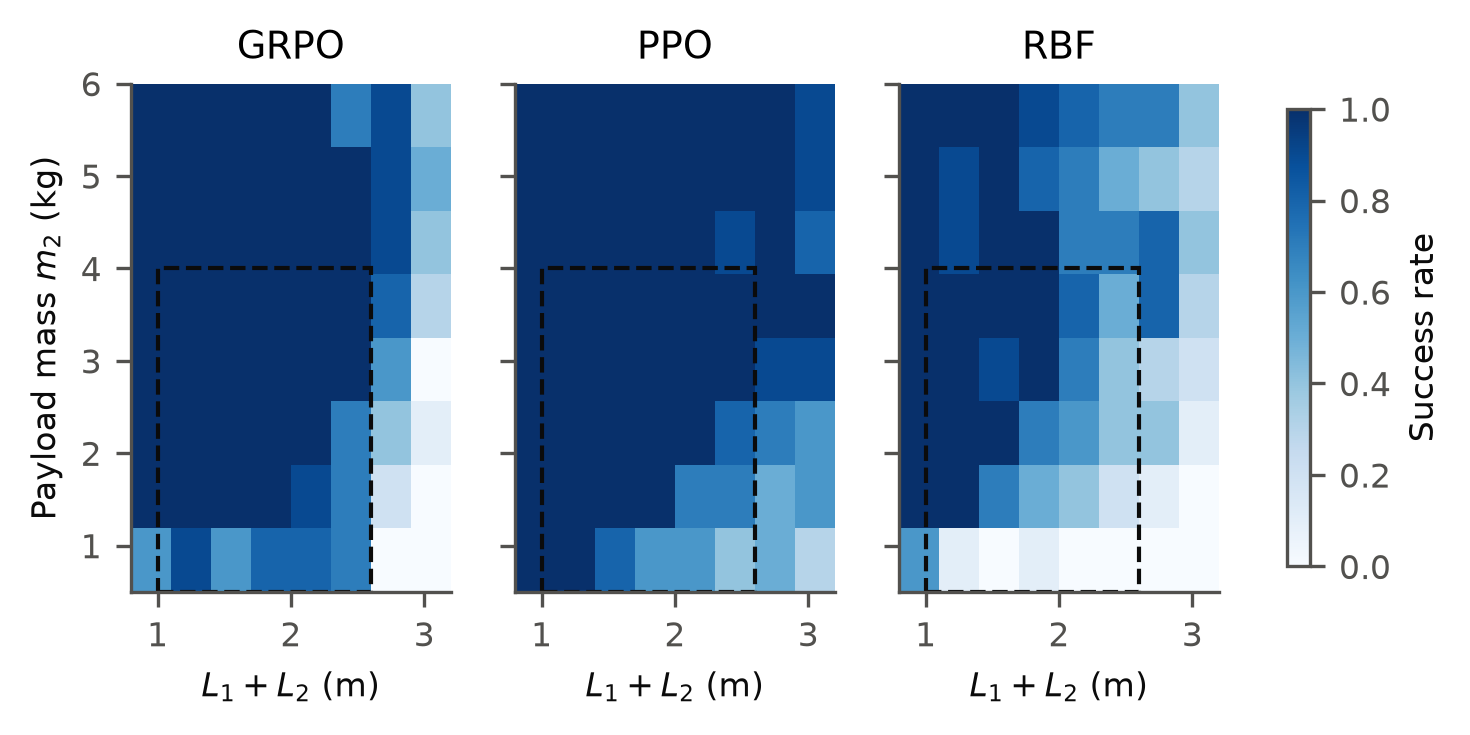
\includegraphics[width=\columnwidth]{robustness_heatmap.png}
\caption{Success rate over payload mass and cable length (10 episodes per cell). The dashed box is the training range.}
\label{fig:heat}
\end{figure}

\begin{figure}[t]
\centering
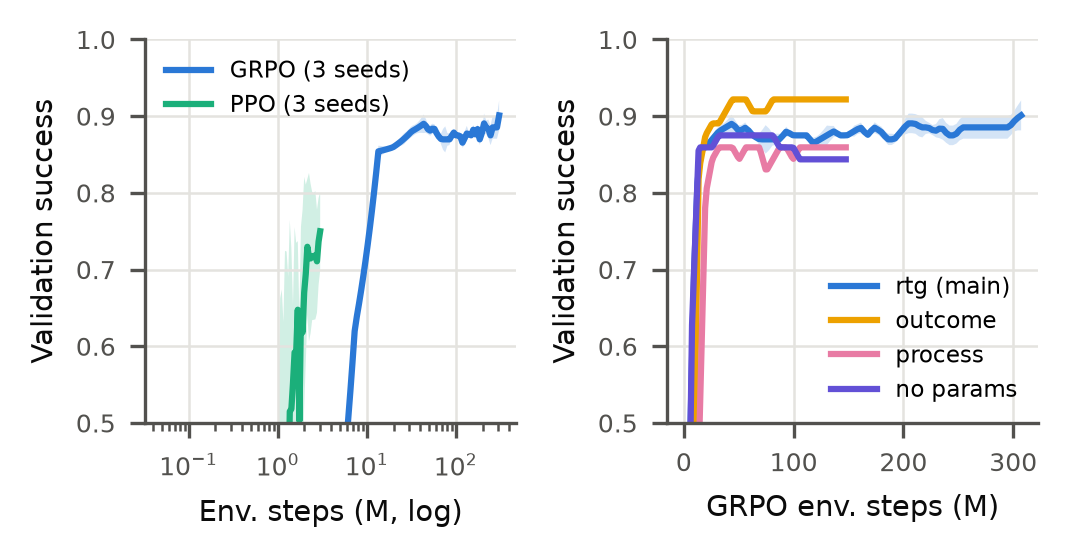
\includegraphics[width=\columnwidth]{learning_curves.png}
\caption{Validation success on 64 held-out scenarios. Left: GRPO vs PPO, mean $\pm$ std over 3 seeds (log steps). Right: GRPO advantage variants and the no-parameter ablation.}
\label{fig:curves}
\end{figure}

\textbf{GRPO vs PPO.} On random scenarios GRPO's three seeds reach 94/93/97\% success and PPO's reach 94/84/77\%. The group baseline gives markedly lower seed-to-seed variance than a learned critic.
\begin{itemize}
\item \emph{Where GRPO is better.} It settles fastest in every condition (7.1\,s vs 7.9\,s on random scenarios) and is clearly more robust to doubled gusts (92\% vs 81\%).
\item \emph{Where PPO is better.} PPO needs $100\times$ fewer samples (3M vs ${\sim}$300M steps; Fig.~\ref{fig:curves}). Batched GPU simulation offsets this: GRPO passes 85\% validation success in about 3\,min on an RTX 3050 Ti laptop GPU. It is smoother (0.5$^\circ$ residual sway, $0.64\times$ GRPO's control energy) and extrapolates better beyond the training range (OOD 96\% vs 81\%; Fig.~\ref{fig:heat}).
\item \emph{Why.} GRPO's Monte-Carlo, scenario-matched baseline is exact for the scenarios it sees. PPO's value function smooths across plants, which helps it extrapolate.
\end{itemize}

\textbf{RL vs RBF.} Both RL agents beat the RBF controller in every condition: 94\% vs 62\% on random scenarios, and 92/81\% vs 48\% under doubled gusts. With only the trolley actuated, the computed-traction law reaches the sway only through the inertia coupling of $M_0(q)$, along a fixed reference. Online RBF adaptation barely helps (57\% with adaptation vs 63\% with $\gamma{=}0$), because compensating model error cannot create the missing actuation. The RBF controller degrades quickly with long cables and light payloads (Fig.~\ref{fig:heat}).

\textbf{Ablations} (Fig.~\ref{fig:curves}; 100 random test scenarios; ablation runs use 120 iterations, the main run 250).

\begin{itemize}
\item \emph{Success saturates for every variant} (rtg 94\%, outcome 96\%, process 95\%), but the return separates them: rtg 61, outcome 45, process $-7$.
\item \emph{The paper's process advantage is worst} (32$^\circ$ peak sway). Its suffix sums over 600 dense steps carry a time-dependent offset shared by every trajectory.
\item \emph{Hiding $(m_2,L_1,L_2)$} keeps 94\% success (return 48). No load cell or rope encoder is needed.
\end{itemize}

\section{Conclusion}
Critic-free GRPO transfers from LLM reasoning to physical control. Replaying each scenario across a group gives a low-variance baseline, which yields the fastest-settling and most gust-robust controller here, consistent across seeds. PPO is more sample-efficient and extrapolates better. Both RL methods clearly beat RBF adaptive control.


\bibliographystyle{IEEEtran}
\begin{thebibliography}{9}
\bibitem{grpo} Z. Shao \emph{et al.}, ``DeepSeekMath: Pushing the limits of mathematical reasoning in open language models,'' arXiv:2402.03300, 2024.
\bibitem{qiang2021} H. Qiang, Y. Sun, J. Lyu, D. Dong, ``Anti-sway and positioning adaptive control of a double-pendulum effect crane system with neural network compensation,'' \emph{Front. Robot. AI}, vol. 8, 639734, 2021.
\bibitem{ppo} J. Schulman \emph{et al.}, ``Proximal policy optimization algorithms,'' arXiv:1707.06347, 2017.
\end{thebibliography}

\end{document}
